Nella fase 4 vengono eseguiti i seguenti incrementi e attività:
\begin{itemize}
	\item Incremento 1
			\begin{itemize}
				\item normazione: modifiche alle \textit{NormeDiProgetto\_v3.0.0} secondo quanto segnalato alla Revisione di Qualifica. Si procede poi con il suo incremento;
				\item pianificazione della qualifica: modifiche al \textit{PianoDiQualifica\_v3.0.0} secondo quanto segnalato alla Revisione di qualifica. Si procede poi con il suo incremento;
				\item pianificazione delle attività: modifiche al \textit{PianoDiProgetto\_v3.0.0} secondo quanto segnalato alla Revisione di Qualifica;
			\end{itemize}
	\item Incremento 2 e Incremento 3
		\begin{itemize}
			\item progettazione di dettaglio: incremento al \textit{Product Baseline} con i requisiti indicati nella tabella 4;
			\item codifica: codifica degli incrementi effettuati durante la progettazione;
			\item redazione manuali: incrementi al \textit{ManualeUtente\_v1.0.0} e al \textit{ManualeSviluppatore\_v1.0.0} in base a quanto segnalato alla Revisione di Qualifica;
			\item verifica: verifica degli incrementi effettuati;
		\end{itemize}
	\item Incremento 4
		\begin{itemize}
			\item Documentazione;
			\item Verifica documentazione;
		\end{itemize}
	\item validazione e collaudo: vengono eseguiti i test di qualifica e il collaudo per il rilascio;
	\item preparazione alla presentazione;
	\item approvazione dei documenti da parte del responsabile. Sono pronti per il rilascio le \textit{NormeDiProgetto\_v4.0.0}, il \textit{PianoDiProgetto\_v4.0.0}, il \textit{PianoDiQualifica\_v4.0.0}, l'\textit{AnalisiDeiRequisiti\_v4.0.0} il
	\textit{ManualeUtente\_v2.0.0} e il \textit{ManualeSviluppatore\_v2.0.0};
\end{itemize}

\begin{tabularx}{\textwidth}{| c | c | }
	\rowcolor{LightBlue}
	\color{white}\bfseries Incremento 1 & 
	\color{white}\bfseries Incremento 2  \\[0.25cm]
	RDF22 & RDF3 \\ 
	RDF23 & RDF4 \\ 
	RDF24 & RDF5 \\ 
	RDF25 & RDF6 \\ 
	RDF26 & RDF7 \\ 
	RDF27 & RDF8 \\ 
	RDF28 & RDF10 \\ 
	RDF29 & RDF11 \\ 
	RDF30 & RDF12 \\ 
	RDF31 & RDF13 \\ 
	RDF32 & RDF14 \\ 
	RDF33 & RDF15 \\ 
	RDF34 & RDF16 \\ 
	RDF35 & RDF17 \\ 
	RDF36 & RDF18 \\
	RDF37 & RDF19\\
	RDF38 & RDF20 \\
	RDF39 & RDF21 \\
	RDF40 &  \\
	RDF41 &  \\
	RDF42 &  \\
	RDF43 &  \\
	RDF44 &  \\
		 \hline
		 \caption{Requisiti da soddisfare in fase 4}
\end{tabularx}

\begin{figure}[h]
	\centering
	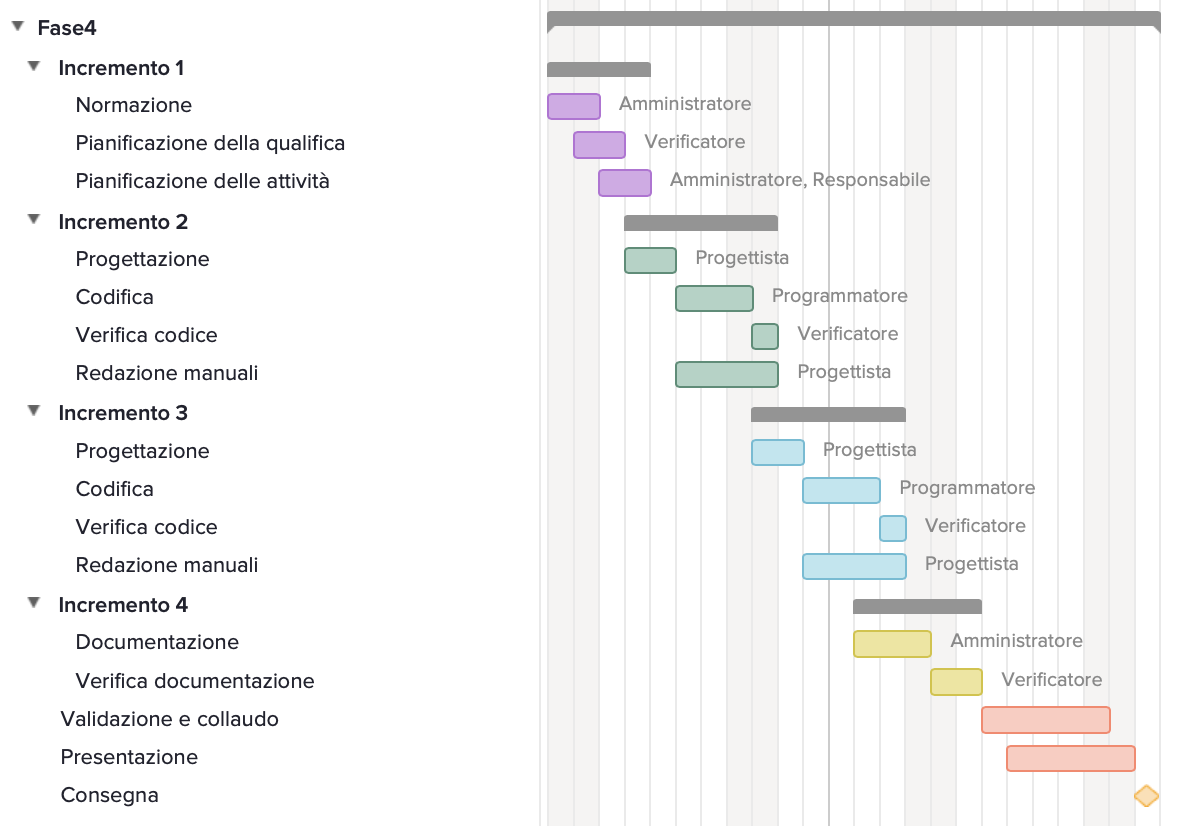
\includegraphics[scale=0.70]{images/fase4.png}
	\caption{Diagramma di Gantt riguardante la fase 4}
\end{figure}